% ----------------------------------------------------------------- %
%             The Speech Signal Processing Toolkit (SPTK)           %
%             developed by SPTK Working Group                       %
%             http://sp-tk.sourceforge.net/                         %
% ----------------------------------------------------------------- %
%                                                                   %
%  Copyright (c) 1984-2007  Tokyo Institute of Technology           %
%                           Interdisciplinary Graduate School of    %
%                           Science and Engineering                 %
%                                                                   %
%                1996-2017  Nagoya Institute of Technology          %
%                           Department of Computer Science          %
%                                                                   %
% All rights reserved.                                              %
%                                                                   %
% Redistribution and use in source and binary forms, with or        %
% without modification, are permitted provided that the following   %
% conditions are met:                                               %
%                                                                   %
% - Redistributions of source code must retain the above copyright  %
%   notice, this list of conditions and the following disclaimer.   %
% - Redistributions in binary form must reproduce the above         %
%   copyright notice, this list of conditions and the following     %
%   disclaimer in the documentation and/or other materials provided %
%   with the distribution.                                          %
% - Neither the name of the SPTK working group nor the names of its %
%   contributors may be used to endorse or promote products derived %
%   from this software without specific prior written permission.   %
%                                                                   %
% THIS SOFTWARE IS PROVIDED BY THE COPYRIGHT HOLDERS AND            %
% CONTRIBUTORS "AS IS" AND ANY EXPRESS OR IMPLIED WARRANTIES,       %
% INCLUDING, BUT NOT LIMITED TO, THE IMPLIED WARRANTIES OF          %
% MERCHANTABILITY AND FITNESS FOR A PARTICULAR PURPOSE ARE          %
% DISCLAIMED. IN NO EVENT SHALL THE COPYRIGHT OWNER OR CONTRIBUTORS %
% BE LIABLE FOR ANY DIRECT, INDIRECT, INCIDENTAL, SPECIAL,          %
% EXEMPLARY, OR CONSEQUENTIAL DAMAGES (INCLUDING, BUT NOT LIMITED   %
% TO, PROCUREMENT OF SUBSTITUTE GOODS OR SERVICES; LOSS OF USE,     %
% DATA, OR PROFITS; OR BUSINESS INTERRUPTION) HOWEVER CAUSED AND ON %
% ANY THEORY OF LIABILITY, WHETHER IN CONTRACT, STRICT LIABILITY,   %
% OR TORT (INCLUDING NEGLIGENCE OR OTHERWISE) ARISING IN ANY WAY    %
% OUT OF THE USE OF THIS SOFTWARE, EVEN IF ADVISED OF THE           %
% POSSIBILITY OF SUCH DAMAGE.                                       %
% ----------------------------------------------------------------- %
\hypertarget{ifft}{}
\name{ifft}{inverse FFT for complex sequence}{signal processing}

\begin{synopsis}
\item[ifft] [ --l $L$ ]  [ --\{ R $|$ I \} ] [ {\em infile} ] 
\end{synopsis}

\begin{qsection}{DESCRIPTION}
{\em ifft} calculates the Inverse Discrete Fourier Transform (IDFT) 
of complex-valued data from {\em infile} (or standard input), 
sending the results to standard output.
The input and output data is in float format, arranged as follows.
\begin{center}
 \leavevmode
 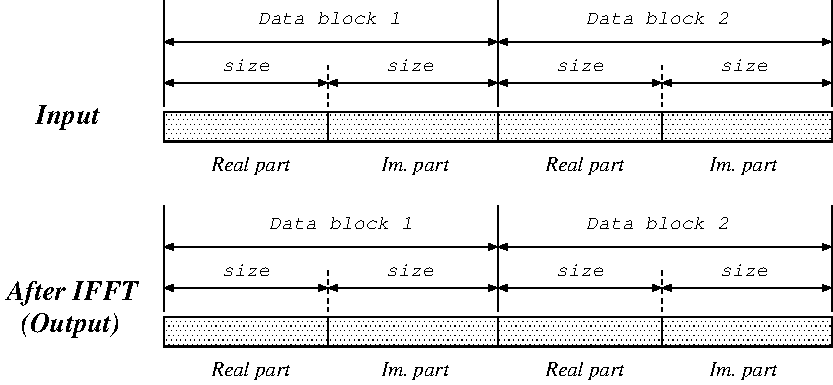
\includegraphics{fig/ifft.pdf} 
\end{center}
\end{qsection}

\begin{options}
	\argm{l}{L}{FFT size power of 2}{256}
	\argm{R}{}{output only real part}{FALSE}
	\argm{I}{}{output only imaginary part}{FALSE}
\end{options}

\begin{qsection}{EXAMPLE}
In this example, the inverse DFT is evaluated from a data file
{\em data.f} in float format
(real part: 256 points, imaginary part: 256 points),
and the output is written to {\em data.ifft}:
\begin{quote}
  \verb!ifft data.f -l 256 > data.ifft!
\end{quote}
\end{qsection}

\begin{qsection}{SEE ALSO}
\hyperlink{fft}{fft},
\hyperlink{fft2}{fft2},
\hyperlink{fftr}{fftr},
\hyperlink{fftr2}{fftr2},
\hyperlink{ifftr}{ifftr}
\hyperlink{ifft2}{ifft2}
\end{qsection}
